\documentclass[11pt]{beamer}

% Beamer style
%\usetheme[secheader]{Madrid}
% \usetheme{CambridgeUS}
\useoutertheme{infolines}
\usecolortheme[rgb={0.65,0.15,0.25}]{structure}
% \usefonttheme[onlymath]{serif}
\beamertemplatenavigationsymbolsempty
%\AtBeginSubsection

% Packages
\usepackage[latin1]{inputenc}
\usepackage{color}
\usepackage{amsmath, amsfonts, amssymb}
\usepackage{marvosym}
\usepackage{graphicx}
\usepackage{/home/robin/LATEX/Biblio/astats}

% Commands
\definecolor{darkred}{rgb}{0.65,0.15,0.25}
\definecolor{darkgreen}{rgb}{0,0.4,0}
%\newcommand{\emphase}[1]{\textcolor{darkred}{#1}}
\newcommand{\Esp}{\mathbb{E}}
\newcommand{\dd}{\text{d}}
\newcommand{\emphase}[1]{{#1}}
\newcommand{\paragraph}[1]{\textcolor{darkred}{#1}}
\newcommand{\refer}[1]{\textcolor{gray}{\footnotesize{[\cite{#1}]}}}
\newcommand{\Refer}[1]{\textcolor{gray}{\footnotesize{[#1]}}}
\newcommand{\ra}{$\emphase{\rightarrow} \;$}

% Names
\newcommand{\chr}{}
\newcommand{\comment}{}
\newcommand{\Pt}{{\widetilde{P}}}
\newcommand{\St}{{\widetilde{S}}}
\newcommand{\Zt}{{\widetilde{Z}}}
\newcommand{\mt}{{\widetilde{m}}}

%====================================================================
\title[Genomic alterations \& OU excursions]{
Recurrent genomic alterations and excursions of Markovian processes
}

\author[S. Robin]{S. Robin}

\institute[AgroParisTech / INRA]{
  \bigskip
 \begin{tabular}{ccccc}
    
\includegraphics[height=.075\textheight]{../FIGURES/LogoINRA-Couleur} & 
    \hspace{.02\textwidth} &
    
\includegraphics[height=.075\textheight]{../FIGURES/logagroptechsolo} & 
    \hspace{.02\textwidth} &
    
\includegraphics[height=.075\textheight]{../FIGURES/logo-ssb} \\ 
  \end{tabular} \\
  \bigskip
  {\normalsize
  \begin{tabular}{l}
  Joint on-going work with \\ 
  L. Decreusefond, M.-P. Etienne, G. Lang, V. Stefanov \& P. Vallois
  \end{tabular} \\~
%     \begin{tabular}{rll}
%     On-going work with & L. Decreusefond, & M.-P. Etienne, \\
%     & G. Lang, & V. Stefanov \\
%     \end{tabular}
    }
  }

  \date[SPA'15, Oxford]{Stoch. Proc. Appli., Oxford, July 2015}

%====================================================================

%====================================================================
%====================================================================
\begin{document}
%====================================================================
%====================================================================

\frame{
%   \vspace{-.1\textheight}
%   \hspace{-.1\textwidth}
%   \includegraphics[width=1.1\textwidth, height=1.1\textheight]{speaker_front_slide_template}
  \includegraphics[width=\textwidth, height=\textheight]{speaker_front_slide_template}
  }

%====================================================================
\frame{\titlepage
  }
  
%====================================================================
\section*{Genomic alterations}
\frame{\frametitle{Genomic alterations}}
  
%====================================================================
\frame{\frametitle{Genomic alterations in cancer cells}

  $$
  \begin{tabular}{cc}
    \onslide+<1->{Normal cell} & \onslide+<2->{Tumor cell} \\
    \onslide+<1->{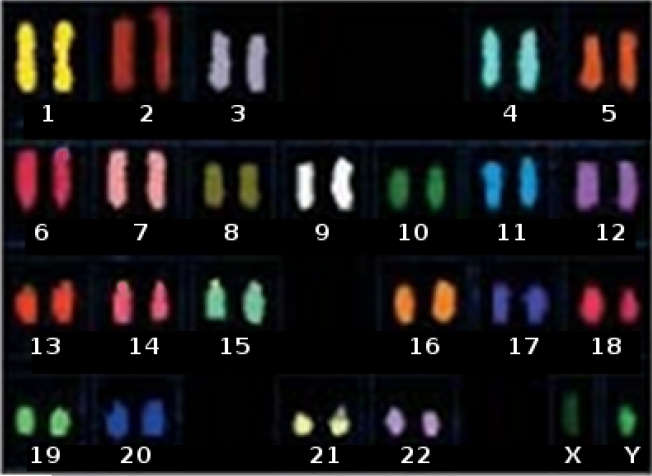
\includegraphics[height=.4\textheight]{../FIGURES/Hup08-Fig121b}}
    &
    \onslide+<2->{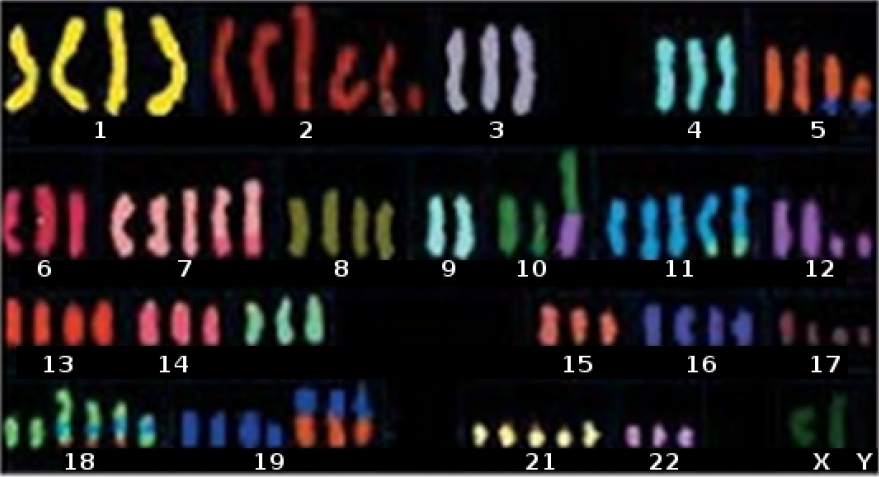
\includegraphics[height=.4\textheight]{../FIGURES/Hup08-Fig121a}}
  \end{tabular}
  $$
  \onslide+<1->{\refer{Hup08}}
}

%====================================================================
\frame{\frametitle{Detection of the alterations}

  $$
  \begin{tabular}{cc}
    \onslide+<2->{CGH profile} & \onslide+<1->{Tumor cell} \\
    \onslide+<2->{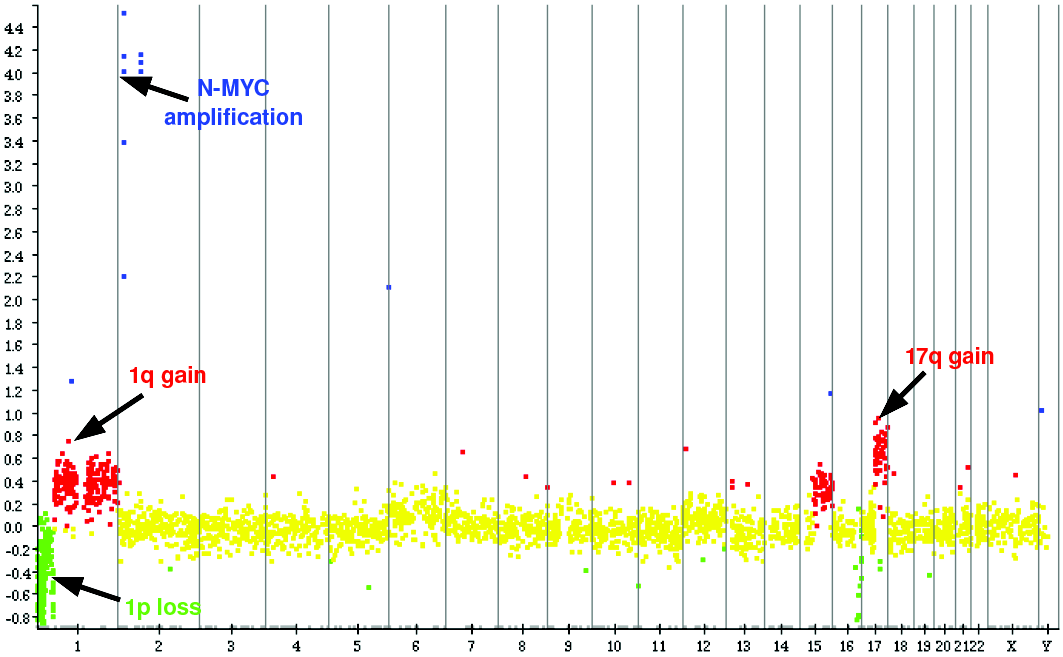
\includegraphics[height=.43\textheight]{../FIGURES/Hup08-Fig128a}}
    &
    \onslide+<1->{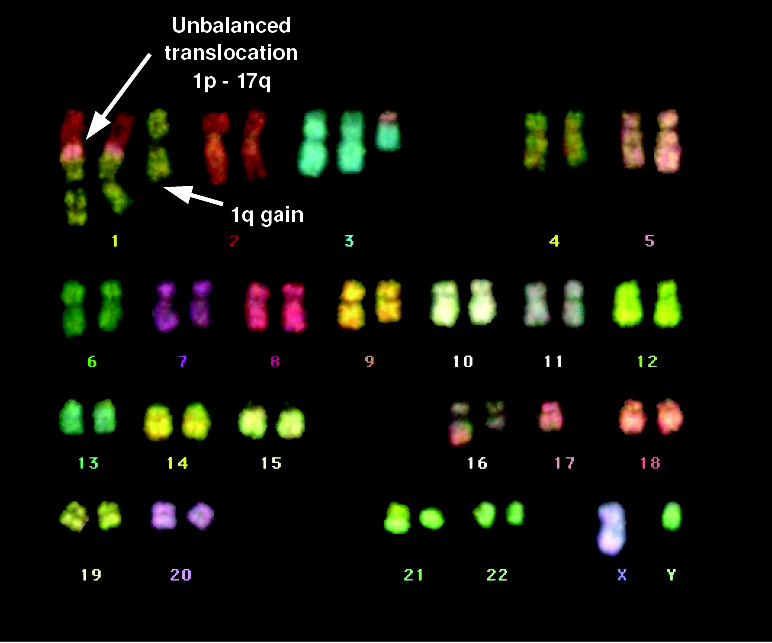
\includegraphics[height=.43\textheight]{../FIGURES/Hup08-Fig128b}}
  \end{tabular}
  $$
  \refer{Hup08}. 

}

%====================================================================
\frame{\frametitle{Recurrent alterations}

  \vspace{-.05\textheight}
  $$
  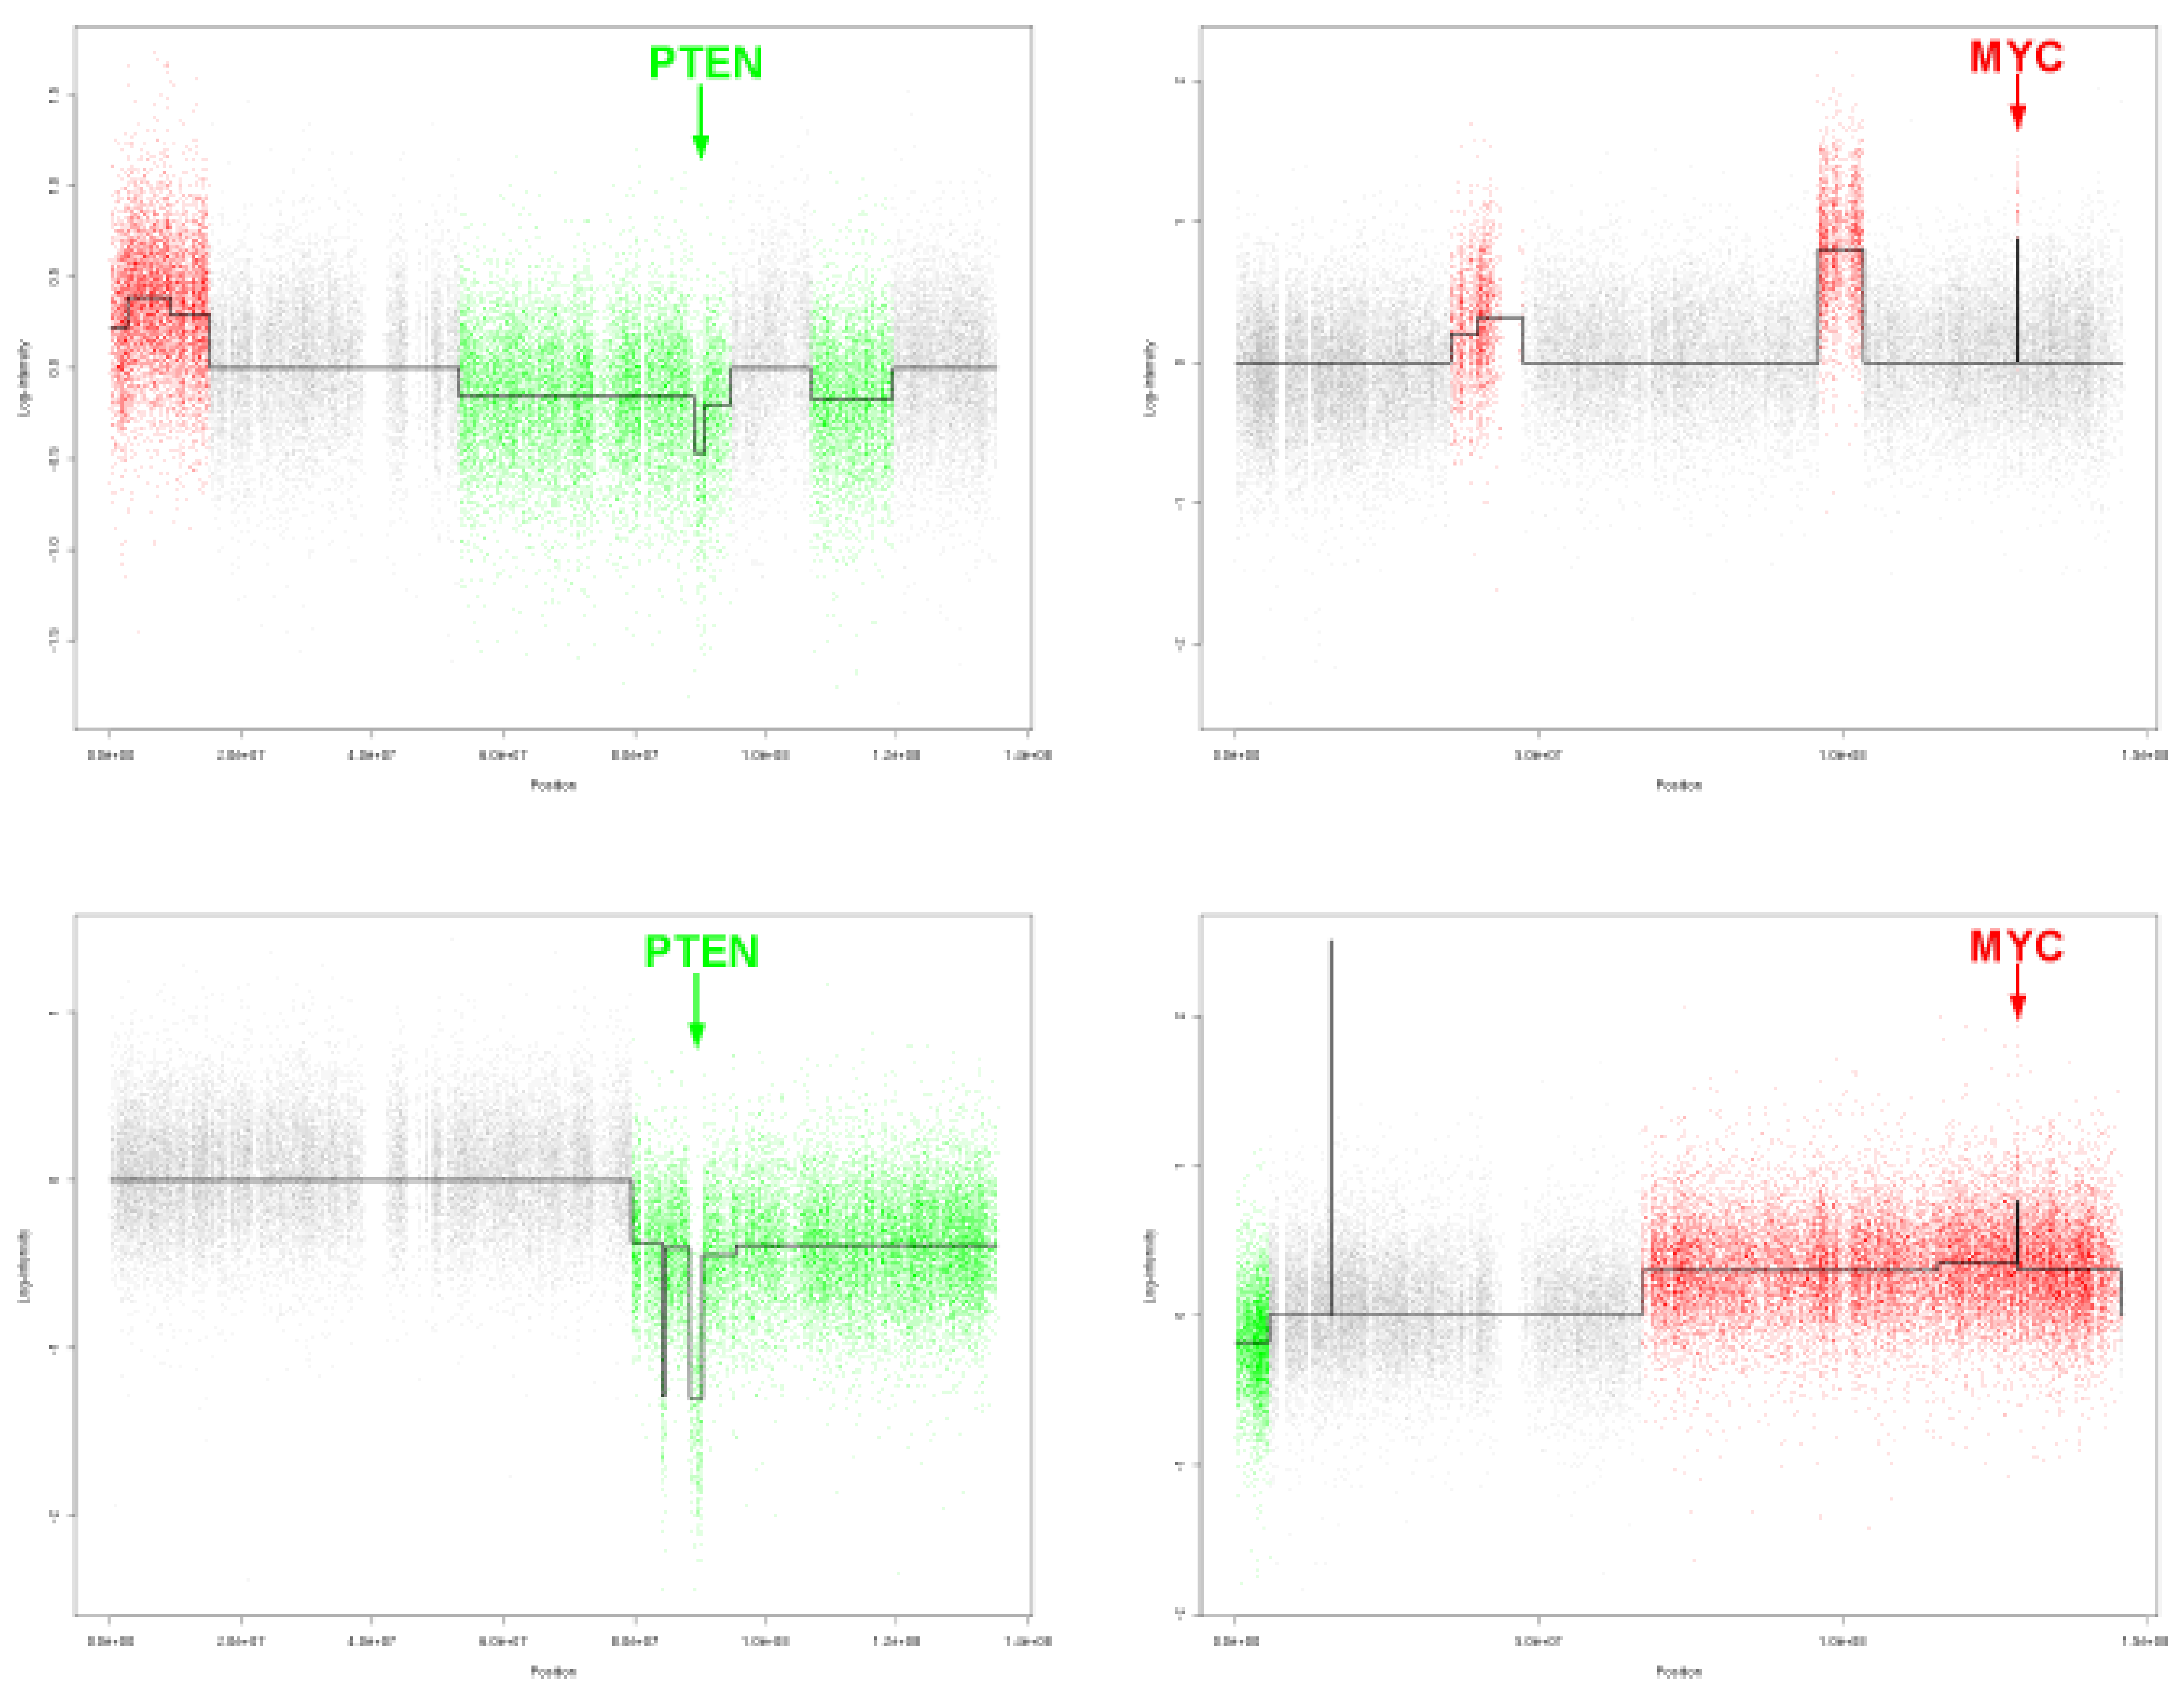
\includegraphics[height=.8\textheight]{../FIGURES/Rig10-Fig6-5}
  $$
  Chrom. 10 and 8 of two patients with breast carcinomas. \refer{Rig11} 
}

%====================================================================
\frame{\frametitle{Profiles}

  \begin{tabular}{cc}
    \begin{tabular}{p{0.5\textwidth}}
    \onslide+<1->{\paragraph{Individual profiles:} 
    patient $i$, locus $t$, 
    $$
    X_i(t) = \left\{
	 \begin{array}{ll}
	 0 & \text{if normal} \\
	 1 & \text{if \textcolor{red}{altered}}
	 \end{array}
    \right.
    $$
   }
    \onslide+<2->{\paragraph{Cumulated profile:}
    $$
    S_p(t) = \sum_{i=1}^p X_i(t)
    $$
    $= $ nb of altered patients at locus $t$ \\
   }
    \onslide+<3->{\bigskip
    \paragraph{Significance:}}
    \end{tabular}
    &
    \hspace{-0.1\textwidth}
    \begin{tabular}{c}
	 \begin{overprint}   
%	 \onslide<1>    
%	 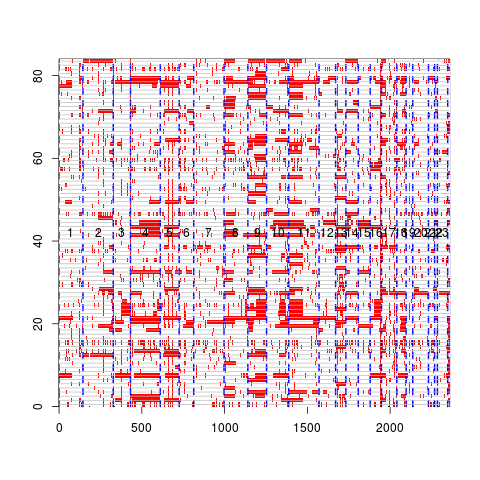
\includegraphics[height=.7\textheight, width=.5\textwidth]{../FIGURES/Fig-MinReg-Data-Prof} 
% 	 \onslide<2>    
% 	 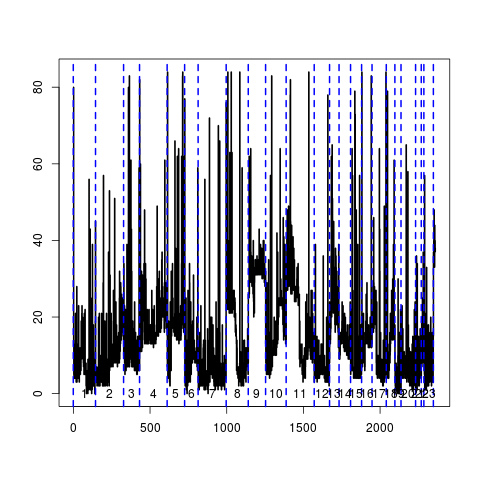
\includegraphics[height=.7\textheight, width=.5\textwidth]{../FIGURES/Fig-MinReg-Data-Cumul} 
	 \onslide<1>    
	 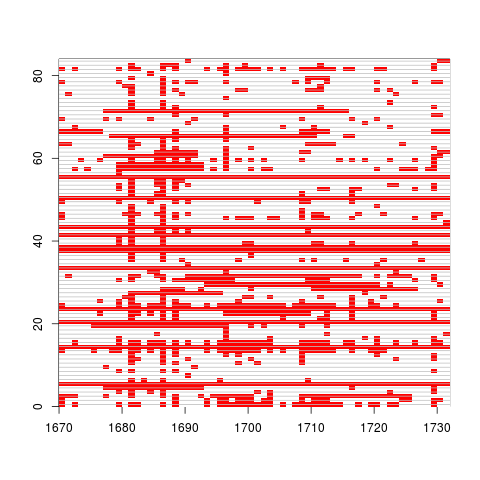
\includegraphics[height=.7\textheight, width=.5\textwidth]{../FIGURES/Fig-MinReg-Data-Prof13} 
	 \onslide<2>    
	 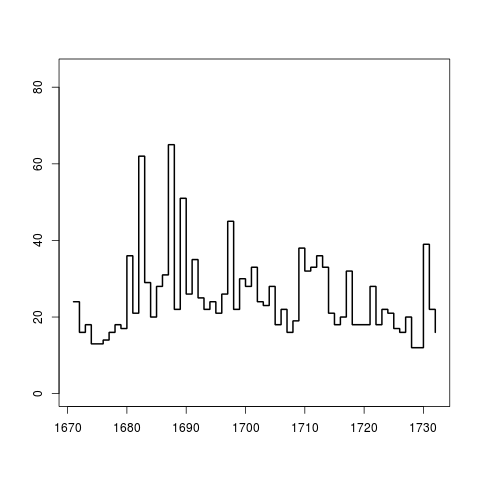
\includegraphics[height=.7\textheight, width=.5\textwidth]{../FIGURES/Fig-MinReg-Data-Cumul13} 
	 \onslide<3>    
	 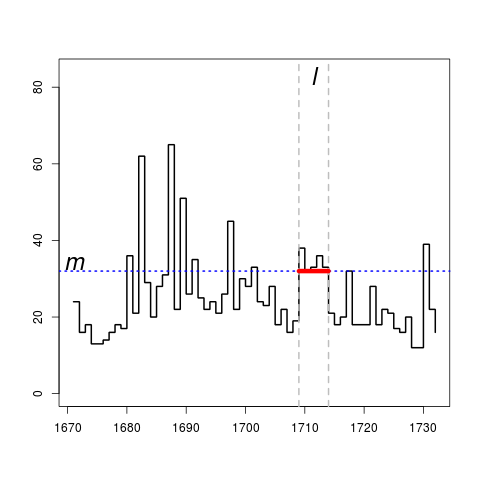
\includegraphics[height=.7\textheight, width=.5\textwidth]{../FIGURES/Fig-MinReg-Data-Reg1-13} 
	 \onslide<4>    
	 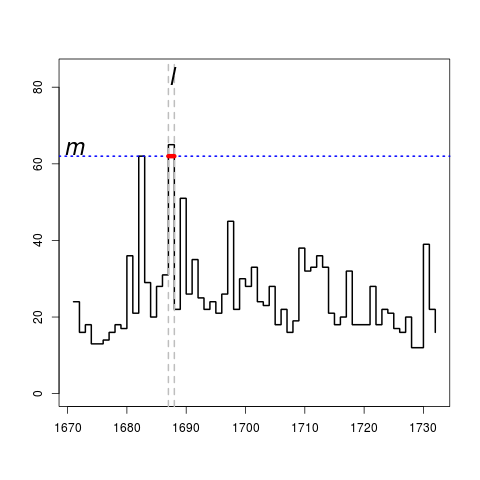
\includegraphics[height=.7\textheight, width=.5\textwidth]{../FIGURES/Fig-MinReg-Data-Reg2-13} 
	 \end{overprint}   
    \end{tabular}
  \end{tabular}
  \onslide+<3->{
  $$
  \pi(m, \ell) = \Pr\left\{\text{
  an excursion with length $\ell$ above level $m$ occurs
  }\right\}
  $$}

  }

%====================================================================
\frame{\frametitle{Generic model}

  \paragraph{Individual profiles.} Define a (Markov) model for each profile $X_i(t)$:
  $$
  X_i(t) \text{ iid } \sim F(\lambda, \mu) 
  $$
  $\lambda, \mu = $ e.g. alteration typical length and frequency.
  
  \bigskip \bigskip \pause
  \paragraph{Cumulated profiles.} Deduce the distribution of $S_p(t)$
  $$
  S_p(t) \sim G(\lambda, \mu)
  $$
  
  \bigskip \pause
  \paragraph{Significance.} Compute the probability for $S_p(t)$ to stay above the threshold $m$ for longer than $\ell$:
  $$
  \pi(m, \ell) =
  \Pr\{\exists t \in ]\ell, n], \forall u \in ]t-\ell, t], S_p(u) \geq m\}
  $$
}

% %====================================================================
% \frame{\frametitle{Abacus}
% 
%   \paragraph{Significance isolines:} for given sample size $p$, number of loci $n$ and parameter $\lambda, \mu \approx $ (mean nb. alterations, mean alteration length)
%   $$
%   \mathcal{C}_\alpha(\lambda, \mu) = \{(m, \ell): \pi(m, \ell) = \alpha\}
%   $$
%   (e.g. $\alpha = 1\%$) \vspace{-.1\textheight}
%   $$
%   \begin{array}{rc}
%     \begin{array}{c} \rotatebox{90}{threshold $m$} \end{array} & 
%     \begin{array}{c} 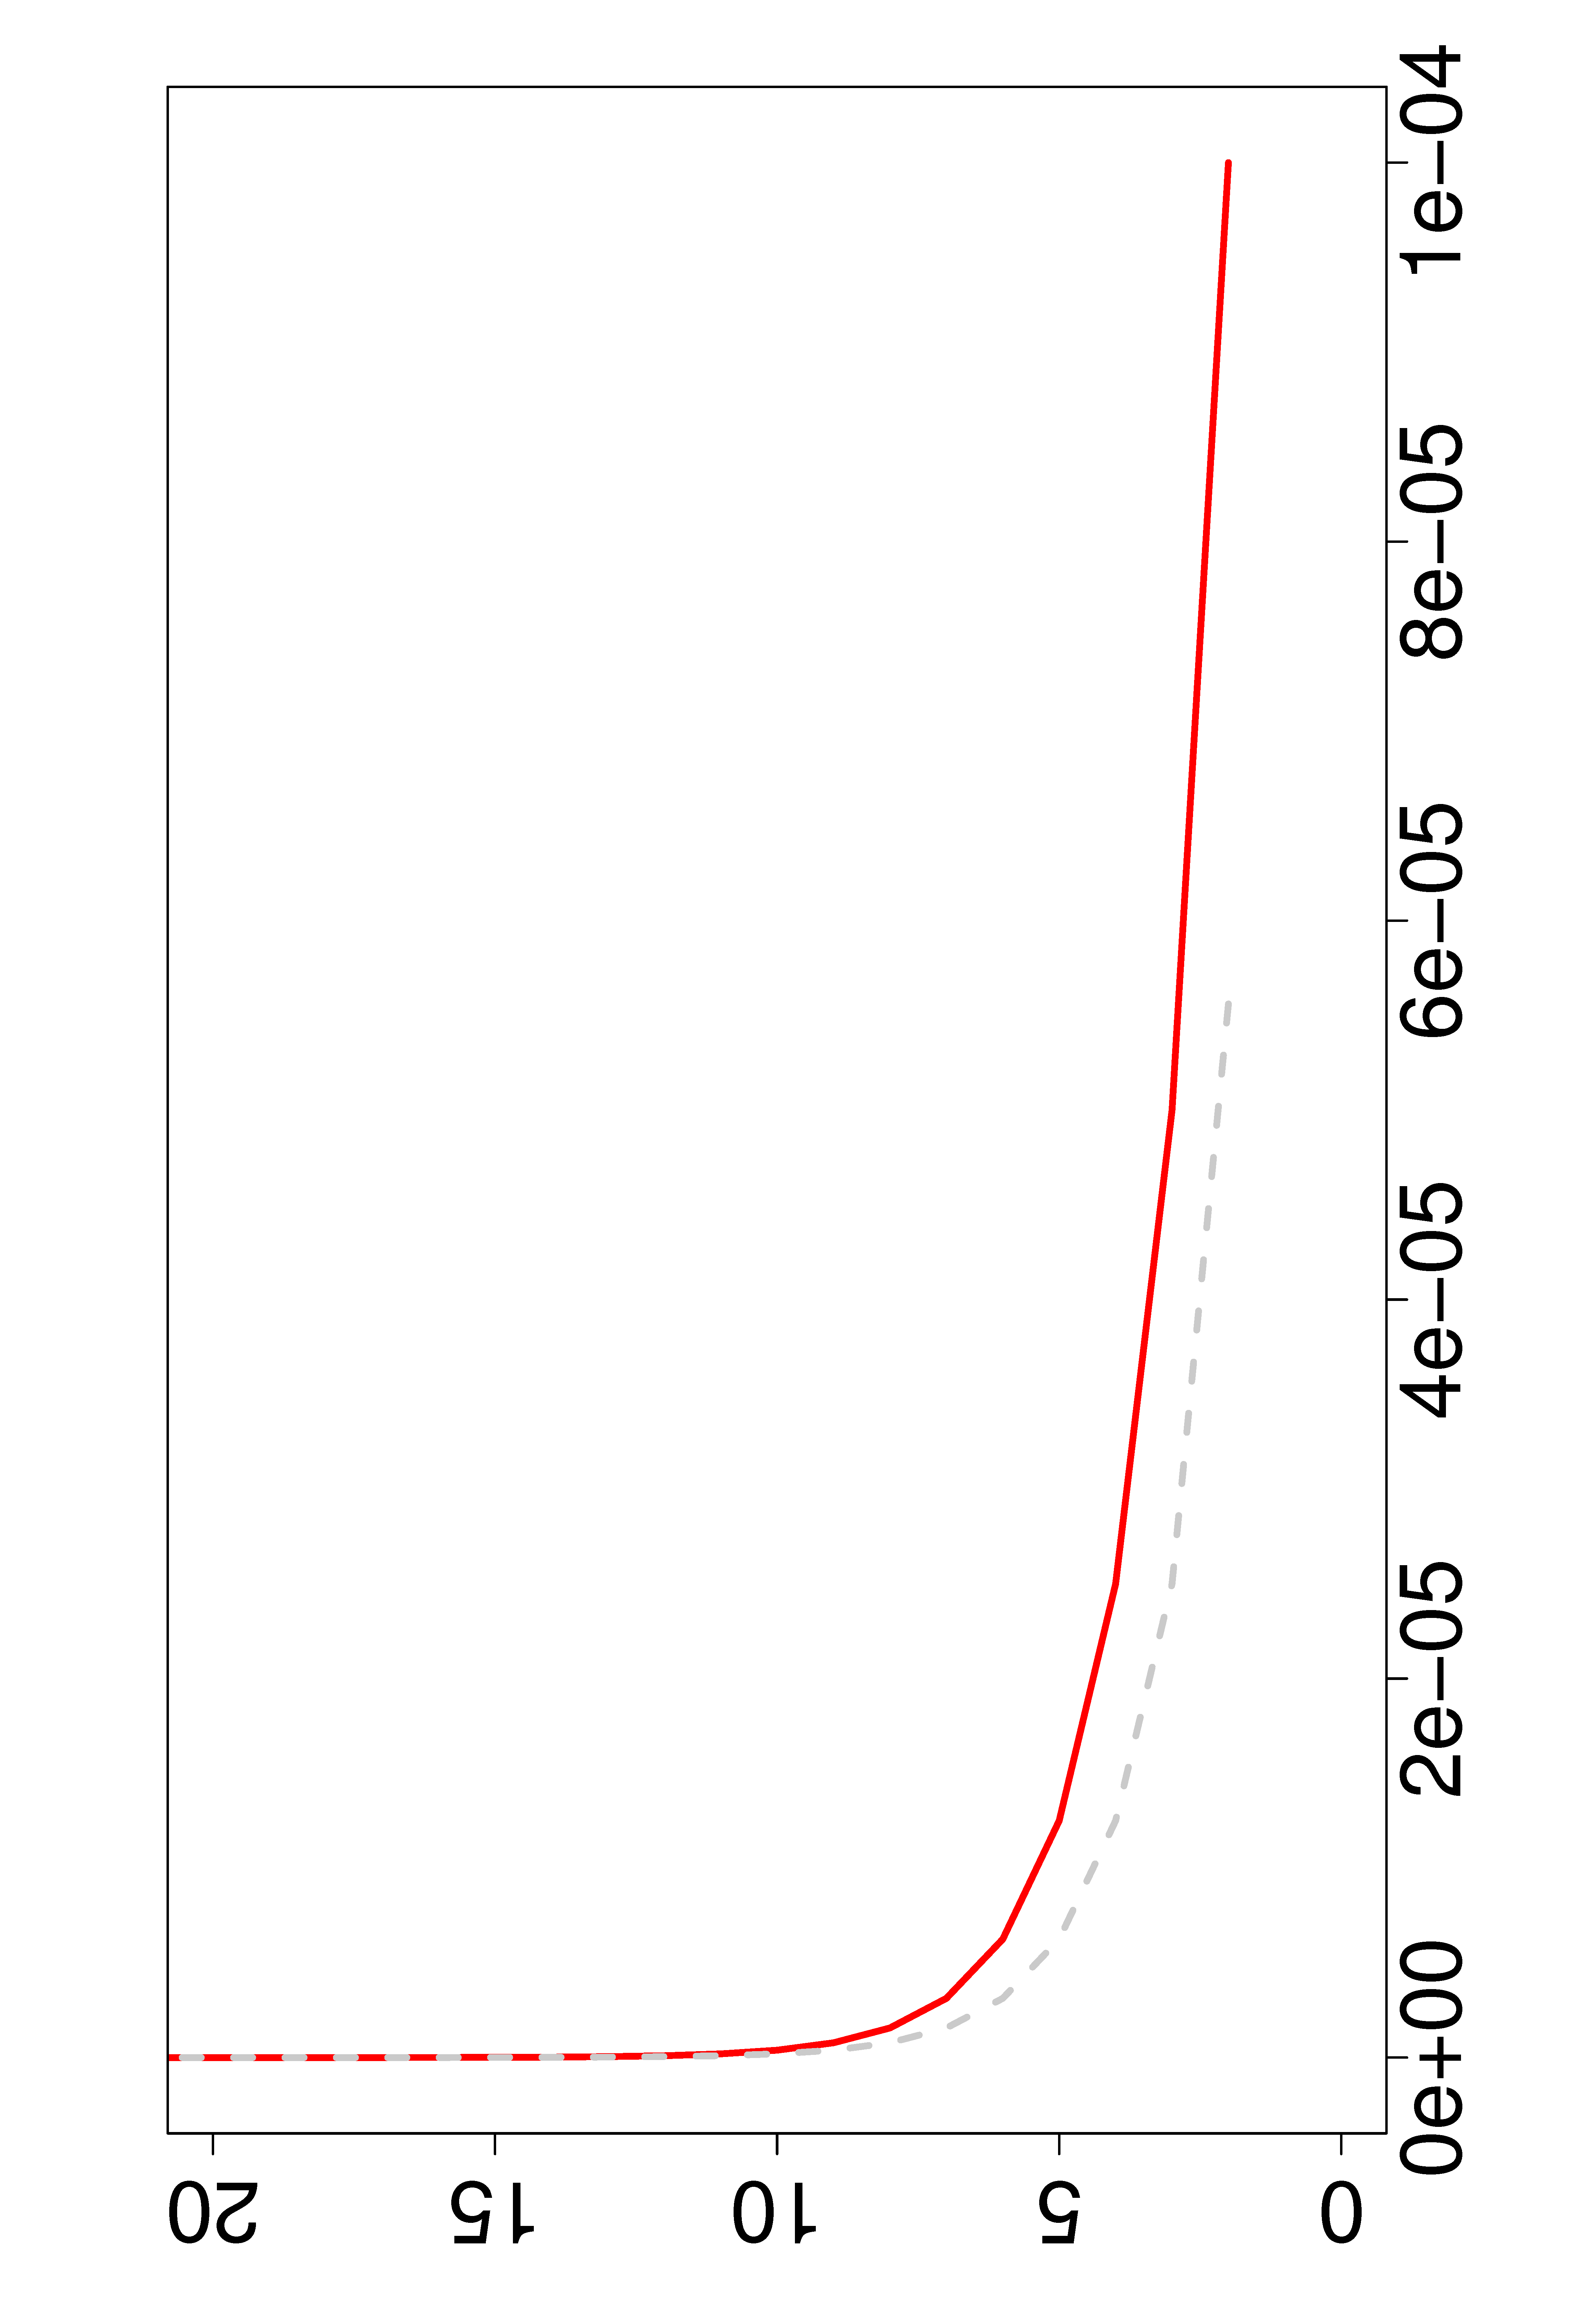
\includegraphics[height=.7\textheight, width=.45\textwidth, angle=270]{../FIGURES/Abaque-Example} \end{array} \\
%     & \text{relative alteration length } \ell / n
%   \end{array}
%   $$
% }

% %====================================================================
% \frame{\frametitle{Outline: A race vs technologies}
%   \tableofcontents
% }

  
%====================================================================
\section{Few loci, few patients}
\frame{\frametitle{Outline} \tableofcontents[currentsection]}
% \frame{\frametitle{Few loci, few patients}}
  
%====================================================================
\frame{\frametitle{Few loci, few patients}

  \paragraph{Mid 90' - early 00':} BAC arrays
  \begin{itemize}
   \item $10^3$ loci per array, $10^2$ loci per chromosome.
%    \item Several k\EUR~per patient
  \end{itemize}
  
  \bigskip
  \paragraph{Data size:} 
  \begin{itemize}
   \item $n \approx 10^2$ loci
   \item $p \approx 10 - 10^2$ patients
  \end{itemize}
  
  \bigskip
  \Refer{R. and Stefanov (2009)}\nocite{RoS09}
}
  
%====================================================================
\frame{\frametitle{Discrete time Markov chain model}

  \paragraph{Individual profile.} $\{X_i(t)\}_i$ iid stationary Markov chains over $\{0, 1\}$:
  $$
  X_i(t) \sim MC(P_X), 
  \qquad
  P_X = \left( 
    \begin{array}{cc} 1 - \lambda & \lambda \\ \mu & 1-\mu \end{array}
  \right).
  $$
  \ra Mean alteration length $= 1/ \mu$, one alteration every $\lambda\mu/(\lambda+\mu)$ locus.
  
  \bigskip \bigskip \pause
  \paragraph{Cumulated profile.} $S_p(t)$ is a Markov chain over $\{0, \dots, p\}$ with transition
  $$
  S_p(t+1) | S_p(t) \quad \overset{\Delta}{=} \quad \underset{\text{stay altered}}{\mathcal{B}\left(S_p(t), 1-\mu \right)} \; + \; \underset{\text{become altered}}{\mathcal{B}\left(p-S_p(t), \lambda \right)}
  $$
  \ra Transition matrix $P_S: (p+1) \times (p+1)$
}

%====================================================================
\frame{\frametitle{Embedded Markov chain}

  \paragraph{Aim = compute $\pi(m, \ell)$.}
  Define the stopping time 
  $$
  T(m, \ell) = \inf\{t: \forall u \in ]t-\ell, t], S_p(u) \geq m\},
  $$
  we have
  $$
  \pi(m, \ell) = \Pr\{T(m, \ell) \leq n\}.
  $$
  
  \bigskip \pause
  \paragraph{Embedded MC principle.} 
  \begin{itemize}
  \item Related to finite automata.
  \item Construct a dedicated Markov chain with enlarged transition matrix $\Pt_S$ and an absorbing state that is reached at $T(m, \ell)$ \refer{FuL03}. 
  \item In this case: relabel the states above $m$ to keep track of how long $S_p(t)$ has sojourned above $m$.
  \end{itemize}
}

% %====================================================================
% \frame{\frametitle{Constructing $\Pt_S$}
% 
% %   \vspace{-.08\textheight}
%   \begin{tabular}{cc}
%     \begin{tabular}{p{0.3\textwidth}}
% 	 \paragraph{Example.}
% 	 $$
% 	 p = 20, m = 15, \ell = 4
% 	 $$
% 
% 	 \onslide+<6->{
% 	 \bigskip
% 	 \paragraph{Result.}
% 	 $$
% 	 \pi(m, \ell) = \left[\Pt_S^{n-1}\right]_{S_p(1), \textcolor{red}{\mathbf{\dagger}}}
% 	 $$
% 	 ($\textcolor{red}{\mathbf{\dagger}} = $ 'coffin state') \\ ~
% 	 \\ ~\\
% 	 or, if $S_p(1) \sim \nu$, \\
% 	 $\pi(m, \ell) = \left[\nu^\top \Pt_S^{n-1}\right]_{\textcolor{red}{\mathbf{\dagger}}}$ 
% 	 }
%     \end{tabular}
%     &
% %    \hspace{-0.05\textwidth}
%     \begin{tabular}{c}
% 	 \begin{overprint}   
% 	 \onslide<1>  
% 	 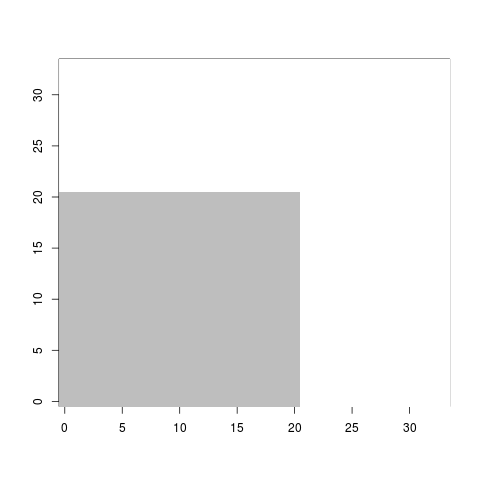
\includegraphics[height=.7\textheight]{../FIGURES/Fig-MinReg-EmbMC-Porg} \\
% 	 {\footnotesize $\{0, \dots, p\}$}
% 	 \onslide<2>    
% 	 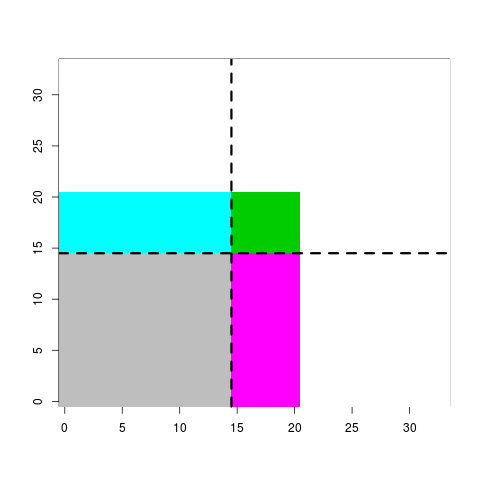
\includegraphics[height=.7\textheight]{../FIGURES/Fig-MinReg-EmbMC-Thres} \\
% 	 {\footnotesize $\{0, \dots, m-1, \underbrace{m, \dots, p}\}$}
% 	 \onslide<3>    
% 	 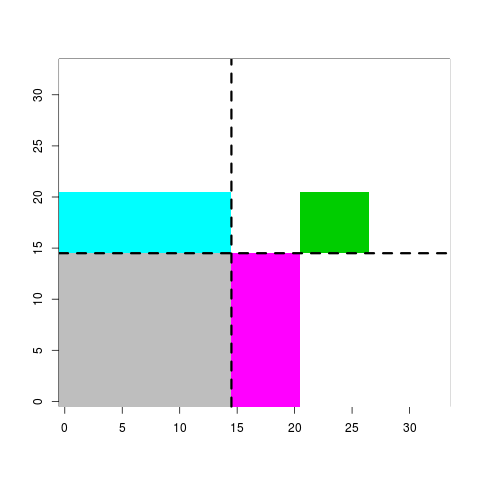
\includegraphics[height=.7\textheight]{../FIGURES/Fig-MinReg-EmbMC-1st} \\
% 	 {\footnotesize $\{0, \dots, m-1, \underbrace{m, \dots, p}, \underbrace{m', \dots, p'}\}$}
% 	 \onslide<4>    
% 	 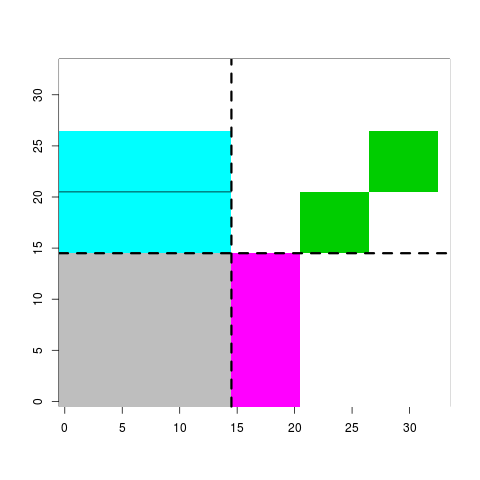
\includegraphics[height=.7\textheight]{../FIGURES/Fig-MinReg-EmbMC-2nd} \\
% 	 {\footnotesize $\{0, \dots, m-1, \underbrace{m, \dots, p}, \underbrace{m', \dots, p'}, \underbrace{m'', \dots, p''}\}$}
% 	 \onslide<5>    
% 	 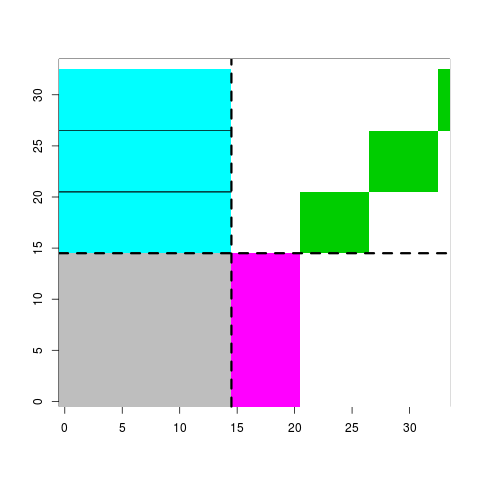
\includegraphics[height=.7\textheight]{../FIGURES/Fig-MinReg-EmbMC-3rd} \\
% 	 {\footnotesize $\{0, \dots, m-1, \underbrace{m, \dots, p}, \underbrace{m', \dots, p'}, \underbrace{m'', \dots, p''}, \textcolor{red}{\mathbf{\dagger}}\}$}
% 	 \onslide<6->   
% 	 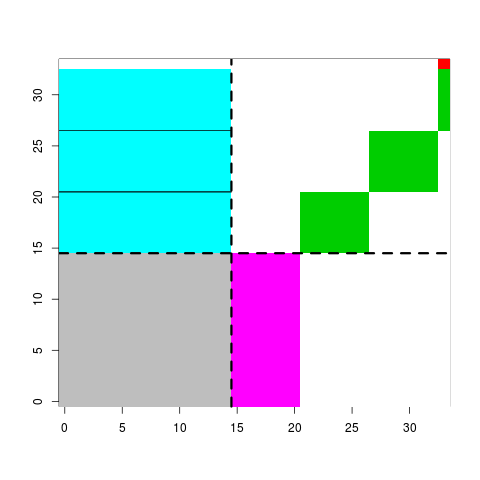
\includegraphics[height=.7\textheight]{../FIGURES/Fig-MinReg-EmbMC-Abs} \\
% 	 {\footnotesize $\{0, \dots, m-1, \underbrace{m, \dots, p}, \underbrace{m', \dots, p'}, \underbrace{m'', \dots, p''}, \textcolor{red}{\mathbf{\dagger}} \}$}
% 	 \end{overprint}   \\~
%     \end{tabular}
%   \end{tabular}
%   
% %   \onslide+<6>{
% % %   \vspace{-0.1\textheight}
% %   \ra Just need to compute $\Pt_S^{n-1}$.
% %   }
% 
%   
% %  \onslide+<7>{
% %  \bigskip 
% %  or, if $S_p(i) \sim \nu$,
% %  $$
% %  \pi(m, \ell) = \sum_s \nu(s) \pi_s(m, \ell) = \left[\nu^\top \Pt_S^{n-1}\right]_{\textcolor{red}{\mathbf{\dagger}}}
% %  $$
% %  }
% 
%   }
% 
%====================================================================
\frame{\frametitle{(Provisional) conclusion}

  \paragraph{Ok:}
  \begin{itemize}
  \item Simple \& intuitive model,
  \item Exact result,
  \item Calculation easy to implement.
  \end{itemize}

  \pause \bigskip \bigskip
  \paragraph{But:}
  \begin{itemize}
  \item The embedded transition matrix $\Pt_S$ has dimension $\approx \ell \times p$ \\
  \ra not tractable for large population size $p$ and/or large alteration length $\ell$
  \item Computing its $(n-1)$-th power leads to numerical troubles for large number of loci $n$. 
  \end{itemize}

  }

%====================================================================
\section{Many loci, few patients}
\frame{\frametitle{Outline} \tableofcontents[currentsection]}
% \frame{\frametitle{Many loci, few patients}}
  
%====================================================================
\frame{\frametitle{Many loci, few patients}

  \paragraph{Mid 00':} %CGH arrays, 
  SNP arrays
  \begin{itemize}
   \item $10^5-10^6$ loci per array, $10^4-10^5$ loci per chromosome.
%    \item Less than 1 k\EUR~per patient
  \end{itemize}
  
  \bigskip
  \paragraph{Data size:} 
  \begin{itemize}
   \item $n \approx 10^4-10^5 \rightarrow \infty$ loci
   \item $p \approx 10^2$ patients
  \end{itemize}
  
  \bigskip
  \Refer{R. and Stefanov (2013)}\nocite{RoS13}
}
  
%====================================================================
\frame{\frametitle{Continuous time Markov process}

  \paragraph{Individual profile.} $\{X_i(t)\}_i$ iid stationary Markov processes over $\{0, 1\}$:
  $$
  \begin{array}{lll}
   \text{rate} & 0 \rightarrow 1: & \lambda, \\
   \text{rate} & 1 \rightarrow 0: & \mu,
  \end{array}
  \qquad \qquad
  X_i(0) \sim \mathcal{B}\left(\frac{\lambda}{\lambda+\mu}\right).
  $$
  \ra Mean alteration length $= 1/ \mu$, alteration frequency $=\lambda\mu/(\lambda+\mu)$.
  
  \bigskip \bigskip \pause
  \paragraph{Cumulated profile.} $S_p(t)$ is a birth and death process over $\{0, \dots, p\}$ with rates
  $$
  \begin{array}{llrcl}
    \text{alteration 'birth'} & s \rightarrow s+1: & \lambda_s & = & \lambda \times (p-s)\\
    \text{alteration 'death'} & s \rightarrow s-1: & \mu_s & = & \mu \times s
  \end{array}
  $$
  \ra infinitesimal generator (transition rates) $Q: (p+1) \times (p+1)$. \\
  \bigskip \pause
  \paragraph{Pb:} The embedded Markov chain approach does not apply anymore.
}

%====================================================================
\frame{\frametitle{Construction of the stopping time}

  \begin{tabular}{cc}
    \begin{tabular}{p{0.3\textwidth}}
 	 \onslide+<1->{$\ell = .05$} \\
 	 \onslide+<2->{$A = T_{S_p(0) \rightarrow m}$} \\
	 \onslide+<3->{$B = (T_{m \rightarrow m-1} | < \ell)$} \\
	 \onslide+<4->{$C = T_{m-1 \rightarrow m}$} \\
    \end{tabular}
    &
    \hspace{-0.1\textwidth}
    \begin{tabular}{p{0.5\textwidth}}
	 \begin{overprint}   
	 \onslide<1>    
	 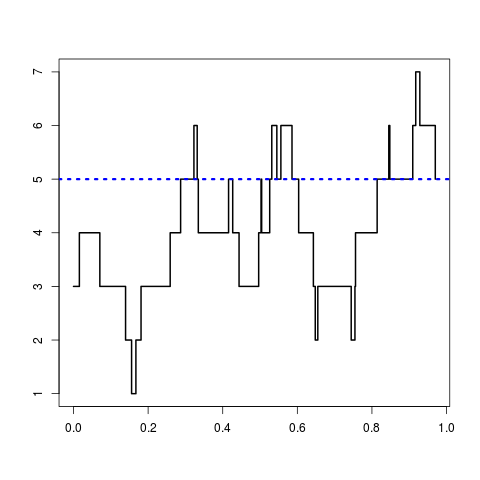
\includegraphics[height=.7\textheight, width=.7\textwidth]{../FIGURES/Fig-MinReg-BirDea-Thres} 
	 \onslide<2>    
	 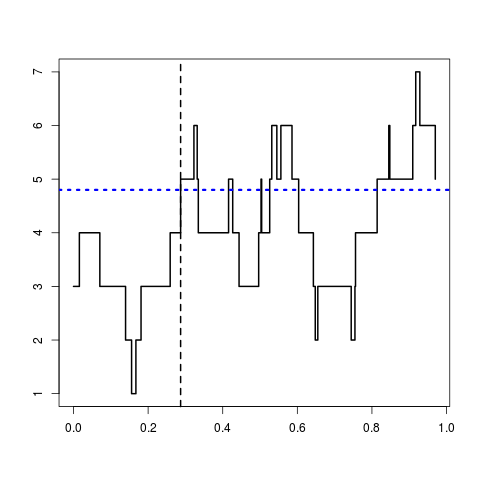
\includegraphics[height=.7\textheight, width=.7\textwidth]{../FIGURES/Fig-MinReg-BirDea-Time1}
	 \onslide<3>    
	 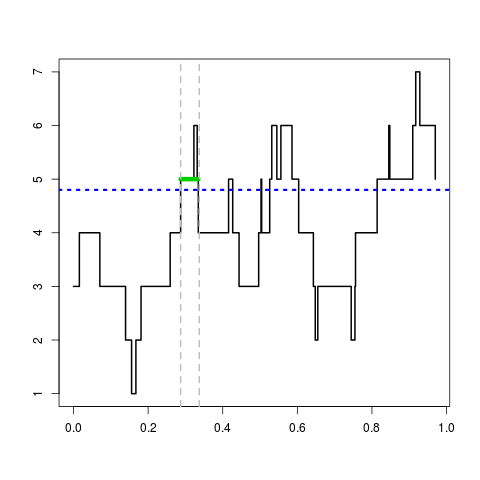
\includegraphics[height=.7\textheight, width=.7\textwidth]{../FIGURES/Fig-MinReg-BirDea-Excur1} 
	 \onslide<4>    
	 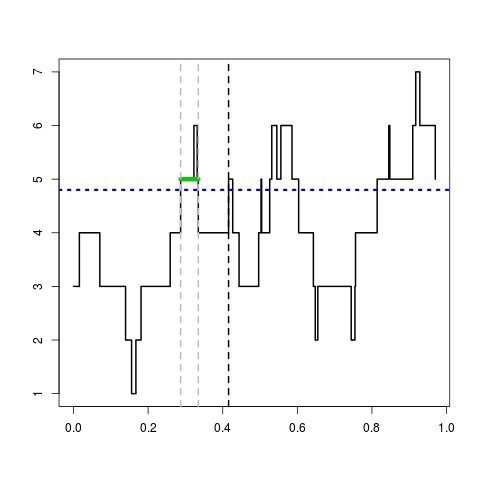
\includegraphics[height=.7\textheight, width=.7\textwidth]{../FIGURES/Fig-MinReg-BirDea-Time2} 
	 \onslide<5>    
	 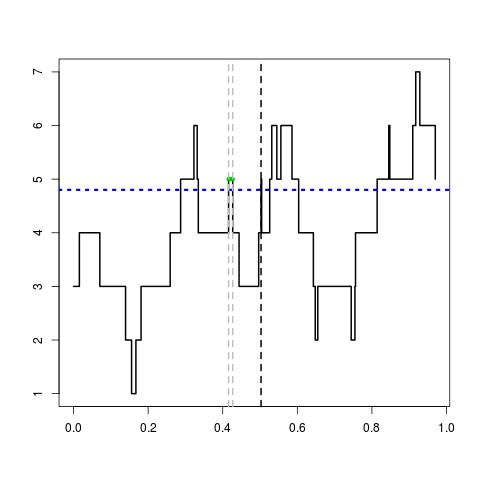
\includegraphics[height=.7\textheight, width=.7\textwidth]{../FIGURES/Fig-MinReg-BirDea-Time3} 
	 \onslide<6>    
	 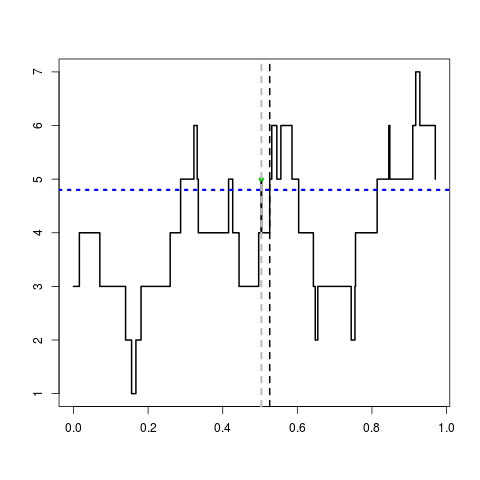
\includegraphics[height=.7\textheight, width=.7\textwidth]{../FIGURES/Fig-MinReg-BirDea-Time4} 
	 \onslide<7>    
	 \includegraphics[height=.7\textheight, width=.7\textwidth]{../FIGURES/Fig-MinReg-BirDea-Time5} 
	 \onslide<8->    
	 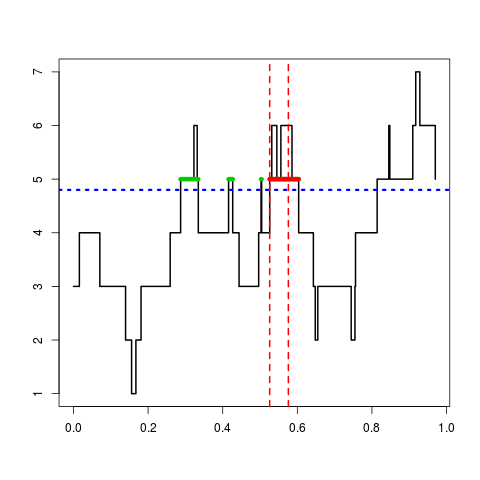
\includegraphics[height=.7\textheight, width=.7\textwidth]{../FIGURES/Fig-MinReg-BirDea-OK} 
	 \end{overprint} 
    \end{tabular}
  \end{tabular}
  \vspace{-.15\textheight}
  \begin{center}
  \onslide+<1->{$T(m, \ell) = $}
  \onslide+<2->{$A$} 
  \onslide+<3->{$+ B_1$} 
  \onslide+<4->{$+ C_1$} 
  \onslide+<5->{$+ (B_2 + C_2)$} 
  \onslide+<6->{$+ (B_3 + C_3)$} 
  \onslide+<7->{$+ (B_4 + C_4)$} 
  \onslide+<8->{$+ \ell$} \\   ~\\
  \end{center}
  \onslide+<8>{Number of trials $\sim$ geometric dist. with parameter $\sigma = \Pr\{T_{m \rightarrow m-1} \geq \ell\}$}
  }

%====================================================================
\frame{\frametitle{Laplace transform of the stopping time}

  \paragraph{Birth and death process.} 
  \begin{itemize}
   \item Hitting time: $T_{a \rightarrow b} = \inf\{t: S_p(t) = b | S_p(0) = a\}$.
   \item \refer{BaS01} provide the Laplace transform of all hitting times $\phi_{T_{a \rightarrow b}}(u)$.
  \end{itemize}

  \bigskip \pause
  \paragraph{Result.} Denoting $\phi_G$ the Laplace transform of $\mathcal{G}(\sigma)$, we have
  $$
  \phi_{T(m, \ell)}(u) = 
  \phi_A(u) 
  \times \phi_G\left\{-\log [
  \phi_{B | < \ell}(u) \; \phi_C(u)
  ] \right\}
  \times e^{-u \ell}
  $$
  and $\Phi_{T(m, \ell)}(u) = \phi_{T(m, \ell)}(u) / u$.

  \bigskip \bigskip \pause 
  \paragraph{Practical calculation.} We are left with the inversion of $\Phi_{T(m, \ell)}$ to get 
  $$
  \Pr\{T(m, \ell) \leq n\} = \Phi^{-1}_{T(m, \ell)}(n),
  $$
  which can be done numerically using e.g. \refer{AbW06}.
}

%====================================================================
\frame{\frametitle{(Provisional) conclusion}

  \paragraph{Ok:}
  \begin{itemize}
  \item Simple \& intuitive model,
  \item Exact result (up the continuous approximation).
  \end{itemize}

  \pause \bigskip \bigskip
  \paragraph{But:}
  \begin{itemize}
  \item The inversion of $\Phi_{T(m, \ell)}$ is numerically unstable \\
  \ra not usable in practice large population size $p$
  \end{itemize}

  }

%====================================================================
\section{Many loci, many patients}
\frame{\frametitle{Outline} \tableofcontents[currentsection]}
% \frame{\frametitle{Many loci, many patients}}
  
%====================================================================
\frame{\frametitle{Many loci, many patients}

  \paragraph{Mid 00':} NGS, DNA-seq
  \begin{itemize}
   \item $10^9$ nucleotides per genome, $10^7-10^8$ nucleotides per chromosome.
%    \item Several tens of \EUR~per patient
  \end{itemize}
  
  \bigskip
  \paragraph{Data size:} 
  \begin{itemize}
   \item $n \rightarrow \infty$ loci
   \item $p \approx 10^3-10^4 \rightarrow \infty$ patients
  \end{itemize}
  
  \bigskip
  \Refer{On-going work: Decreusefond\footnote{from TelecomParisTech}, Etienne, Lang, R., Vallois}
}
  
%====================================================================
\frame{\frametitle{Convergence to an Ornstein-Uhlenbeck process}

\paragraph{Model.} Same model as previously, letting $p$ go to infinity.
$$
S_p(t) = \sum_{i=1}^p X_i(t).
$$

\bigskip \pause 
\paragraph{Proposition.} 
{\sl Denoting $\tau = \lambda + \mu$, $\theta = \lambda/\tau$, $\sigma^2 = \theta(1-\theta)$,
$$
\St_p(t) := \frac{S_p(t) - p \theta}{\sigma \sqrt{p}} 
\quad \overset{\Delta}{\underset{p \rightarrow \infty}{\longrightarrow}} \quad 
Z(t)
$$
where $Z(t) \sim OU(\tau)$ is a stationary Ornstein-Uhlenbeck process with zero mean, unit variance and recall parameter $\tau$ (drift = $-\tau Z(t) \dd t$).
% \begin{eqnarray*}
%   Z(0) & \sim & \mathcal{N}(0, 1), \\
%   \dd Z(t) & = & -\tau Z(t) \dd t + \dd B(t) / \sqrt{1 - e^{-2\tau}}. 
% \end{eqnarray*}
}
}

%====================================================================
\frame{\frametitle{Convergence of the longest excursion}

  \paragraph{The longest excursion} is not a continuous function of the path, so sufficient to guaranty the convergence in distribution so 
  $$
 \St_p(t) \overset{\Delta}{\longrightarrow}
  OU(\tau)
  $$
  is not sufficient to prove that 
  $$
  V^{(1)}_{\St_p} \overset{\Delta}{\longrightarrow} V^{(1)}_{OU(\tau)}.
  $$
  
  \bigskip \pause
  Still, denoting $\St_p^{-\ell}(t) = \min_{t-\ell \leq u \leq t} \St_p(u)$, we have that
  $$
  \pi(m, \ell) = 
  \Pr\left\{\max_{\ell \leq t \leq n} \St_p^{-\ell}
  (t) \geq \mt\right\}
  $$  
  so the convergence of $V^{(1)}_{\St_p}$ holds.
}

%====================================================================
\frame{\frametitle{New problem}

  Denote $V^{(1)}_{OU}(\mt)$ the longest excursion of an $OU(\tau)$ above threshold $\mt$:
  $$
  \pi(m, \ell) = \Pr\{V^{(1)}_{OU}(\mt) \geq \ell\}, \qquad \mt = (m-p\theta)/\sigma\sqrt{p}.
  $$
  \vspace{-.075\textheight}
  \centerline{
%   \begin{tabular}{cc}
%     \begin{tabular}{p{0.4\textwidth}}
%     \end{tabular}
%     &
%     \hspace{-0.05\textwidth}
%     \begin{tabular}{p{0.5\textwidth}}
	 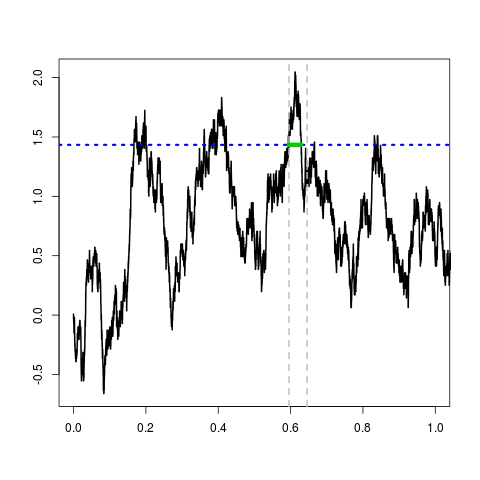
\includegraphics[height=.65\textheight, width=.7\textwidth]{../FIGURES/Fig-MinReg-Diffus-Longest} 
%     \end{tabular}
%   \end{tabular}
  }
  
  \pause
  \paragraph{Pb:} Very few is known about $V^{(1)}_{OU}(\mt)$ for $\mt \neq 0$.

  }

%====================================================================
\frame{\frametitle{First approach: Discrete time sampling}

  \paragraph{Property.} For any $N$, denoting $\delta = n/N$, the discrete time process
  $$
  \left\{ \St(k \delta) \right\} _{k = 0, 1, \dots N}
  $$
  is a first order autoregressive process $AR_1(\phi)$ with autocorrelation parameter $\phi = e^{-\tau \delta}$.
  
  \bigskip \bigskip \pause
  \paragraph{First sampling strategy.}
  \begin{itemize}
  \item Sample a large number $M$ of $AR_1(e^{-\tau \delta})$;
  \item Get the empirical distribution of the largest excursion above $\mt$.
  \end{itemize}
  \bigskip
  \ra Distance between the distribution of the largest discrete excursion and the largest continuous one (depending on $N$ or $\delta$)? \\
  On-going work by T. Boudinar.

}

%====================================================================
\frame{\frametitle{Second approach: Importance sampling}

  We are interested in the expectation of a function 
  $$
  f = f(Z) = f\left(Z(0), T_\mt, V^{(1)}, \varepsilon^{(1)}\right).
  $$
  Provide that $Q \gg P$, 
  \begin{eqnarray*}
  \Esp_P[f(Z)] & = & \Esp_Q\left[f(Z) \frac{\dd P(Z)}{\dd Q(Z)}\right] \\
  & = & \Esp_Q\left[\Esp_Q\left\{f(Z) \frac{\dd P(Z)}{\dd Q(Z)}
  \left| Z(0), T_\mt, \left(V_\mt^{(j)}\right), \left(\varepsilon^{(j)}\right), Z_\mt^{me} \right.\right\}\right]
  \end{eqnarray*}
  where
  \begin{eqnarray*}
  \left(V_\mt^{(j)}\right) & = & \text{ordered lengths of the excursions apart from $\mt$;} \\
  \left(\varepsilon^{(j)}\right) & = & \text{their respective signs;} \\
  Z_\mt^{me} & = & \text{the final meander apart from $\mt$.}
  \end{eqnarray*}
  }

% %====================================================================
% \frame{\frametitle{Second approach: Importance sampling}
%   \paragraph{Monte-Carlo.} For any measurable function $f$, an unbiased estimate of 
%   $
%   \Esp_P[f(X)] = \int f(X) \dd P(X)
%   $
%   is given by
%   $$
%   \widehat{\Esp}_P[f(X)] = \sum_j \frac1M f(X^j) 
%   \qquad \text{with} \quad
%   (X^j)_{j = 1 \dots M} \text{ iid } \sim P.
%   $$
%   
%   \pause \bigskip \bigskip
%   \paragraph{Importance sampling.} When sampling from $P$ is not possible, provided that $Q \gg P$, an alternative estimate is given by
%   \begin{eqnarray*}
%      \widehat{\Esp}_P[f(X)] & = & \sum_j w_j f(X^j) 
%      \qquad \text{with} \quad 
%      (X^j)_{j = 1 \dots M} \text{ iid } \sim Q 
%      \\
%      w_j & = & W_j / \sum_k W_k, 
%      \qquad W_j = \frac{\dd P(X^j)}{\dd Q(X^j)}.
%   \end{eqnarray*}
% }
% 
%====================================================================
\frame{\frametitle{Second approach: Importance sampling}

  \paragraph{Brownian motion starting from 0:} \refer{PiY97} provide a (simple) way to sample 
  \begin{itemize}
   \item the ordered lengths of the excursions apart from 0 $V^{(1)}_B \geq V^{(2)}_B \geq \dots$, 
   \item the signs of the respective excursions $\varepsilon^{(1)}_B, \varepsilon^{(2)}_B, \dots$,
   \item the length and sign of the final meander $B^{me}$.
  \end{itemize}
% as a function of i.i.d. exponential variables $(U_1, U_2, \dots)$:
%   can be sampled as follows:
%   \begin{enumerate}
%   \item Sample $(U_1, U_2, \dots)$ i.i.d. $\sim \mathcal{E}(1)$,
%   \item Compute their cumulated sums: $C_n = U_1 + \dots + U_n$,
%   \item Compute
%   $$
%   V^{(1)}_B = \frac{C_1^{-2}}{\sum_{j \geq 1} C_j^{-2}}, \quad
%   V^{(2)}_B = \frac{C_2^{-2}}{\sum_{j \geq 1} C_j^{-2}}, \quad
%   \dots
%   \text{ where } C_n = \sum_{j=1}^n U_j.
%   $$
%   \end{enumerate}

  \bigskip \pause
  \paragraph{From Brownian excursions to OU excursions.}
  \begin{itemize}
   \item \cite{APP05} provide the distribution of the hitting time $T_{\mt}$ for an OU process.
   \item The Girsanov formula for the rest of the path ($t > T_{\mt}$) can be derived:
   $$
   \left.\frac{\dd P_{OU}}{\dd P_B}\right|_{\mathcal{F}_{T_{\mt}}} = f(V_B^{(1)}, V_B^{(2)}, \dots, \varepsilon^{(1)}_B, \varepsilon^{(2)}_B, \dots, B^{me})
   $$
   \item No need to sample the whole path (except $B^{me}$).
  \end{itemize}
}

% %====================================================================
% \frame{\frametitle{Importance sampling}
% 
% \onslide+<1->
% {We know how to sample $V^{(n)}_B$ but not \textcolor{red}{$V^{(n)}_{OU}$}. \\}
% 
%   \begin{tabular}{cc}
%     \begin{tabular}{p{.4\textwidth}}
% 	 \begin{enumerate}
% 	 \onslide+<2->
% 	 {\item Sample a large number $N$ of copies $V^{(n)}_{B, 1}$, $V^{(n)}_{B, 2}$, \dots, $V^{(n)}_{B, N}$. \\ ~}
% 	 \onslide+<3->
% 	 {\item Reweight each $V_{B, j}$ with 
% 	 $$
% 	 w_j \propto \textcolor{blue}{{\dd P_{OU}}/{\dd P_B}(V_{B, j})}.
% 	 $$}
% 	 \end{enumerate}
% 	 \onslide+<4->
% 	 {$$
% 	 \widehat{\pi}(m, \ell) = \frac{\sum_j w_j \mathbb{I}\{W_{B, j} > \ell\}}{\sum_j w_j}
% 	 $$}
%     \end{tabular}
%     &
%     \hspace{-.05\textwidth}
%     \begin{tabular}{c}
%      \begin{overprint}
%       \onslide<1>
%      	 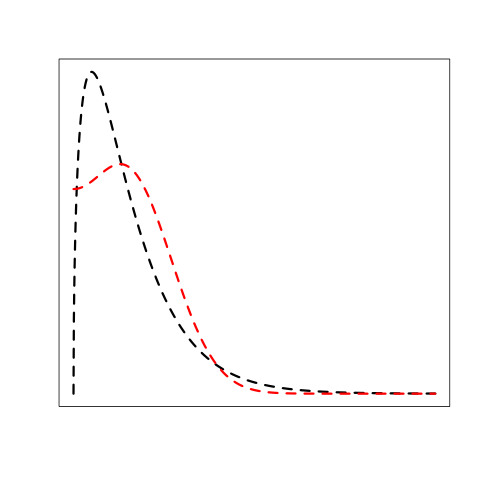
\includegraphics[scale=.4]{../FIGURES/Fig-MinReg-Diffus-ImpSamp0} 
%       \onslide<2>
%      	 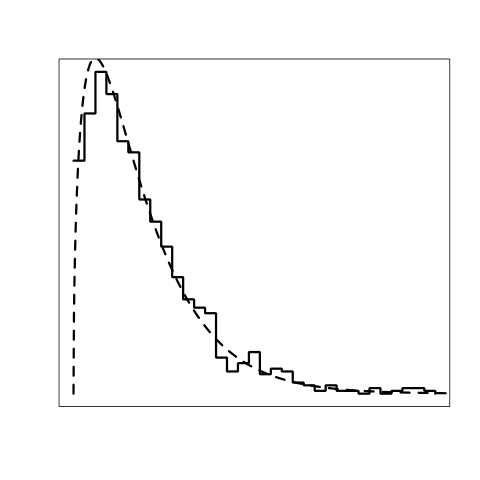
\includegraphics[scale=.4]{../FIGURES/Fig-MinReg-Diffus-ImpSamp2} 
%       \onslide<3>
%      	 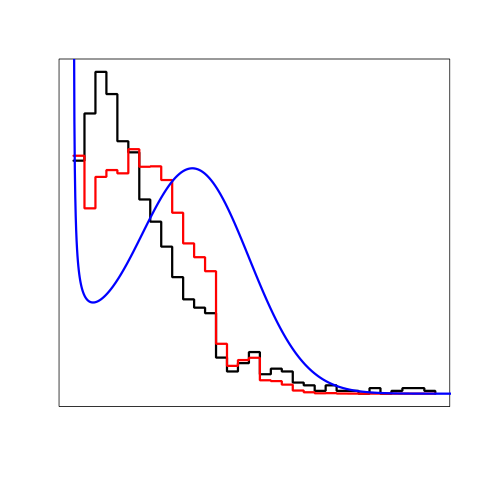
\includegraphics[scale=.4]{../FIGURES/Fig-MinReg-Diffus-ImpSamp3} 
%       \onslide<4->
%      	 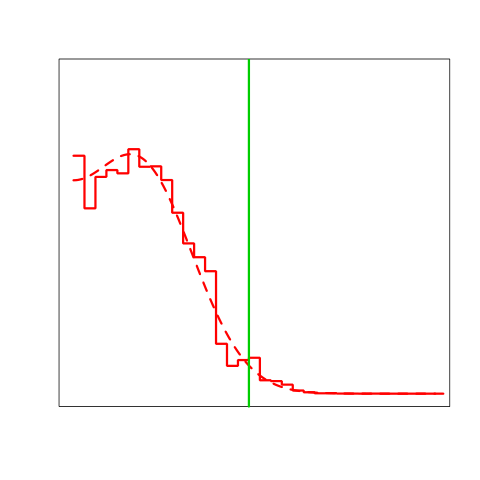
\includegraphics[scale=.4]{../FIGURES/Fig-MinReg-Diffus-ImpSamp4} 
%      \end{overprint}
%     \end{tabular}
%   \end{tabular}
%   
% %   \vspace{-.05\textheight}
% %   \onslide+<5>{A sampling scheme can be designed to sample $OU$ excursions.}
% 
% }
% 
% %====================================================================
% \frame{\frametitle{A theoretical issue}
% 
%   \vspace{-.05\textheight}
%   \begin{tabular}{cc}
%     \begin{tabular}{p{.4\textwidth}}
% 	 \paragraph{The longest excursion} is not a continuous function so 
% 	 $$
% 	 \St_p \overset{\Delta}{\longrightarrow} OU(\tau)
% 	 $$
% 	 is not enough to prove that 
% 	 $$
% 	 V^{(1)}_{\St_p} \overset{\Delta}{\approx} V^{(1)}_{OU(\tau)}.
% 	 $$
%     \end{tabular}
%     &
%     \hspace{-.1\textwidth}
%     \begin{tabular}{c}
%      	 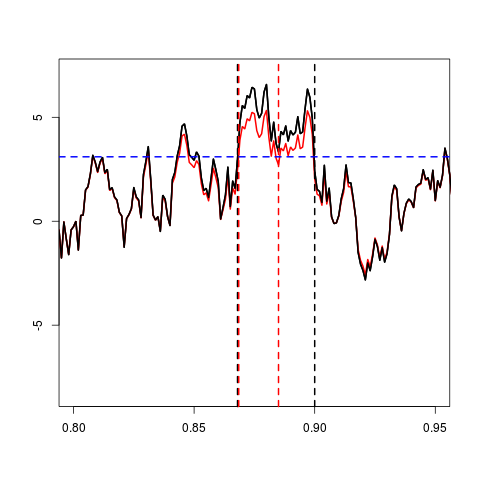
\includegraphics[width=.6\textwidth, height=.55\textheight]{../FIGURES/Fig-MinReg-Diffus-Continuity}      
%     \end{tabular}
%   \end{tabular} \\
%   \pause
%   Still, the problem can be reformulated as
%   $$
%   \pi(m, \ell) = \Pr\left\{\max_{\ell \leq t \leq n} \St_p^{-\ell}(t) \geq \mt\right\}
%   $$
%   where $\St_p^{-\ell}(t) = \min_{t-\ell \leq u \leq t} \St_p(u)$, which relies on continuous transforms\footnote{Many thanks to P. Vallois.}.
%   
% %   $\St_p \overset{\Delta}{\longrightarrow} OU(\tau)$
% %   means that, for any continuous function $f$:
% %   $$
% %   \mathbb{E}[f(\St_p)] \underset{p \rightarrow \infty}{\longrightarrow}  \mathbb{E}[f(OU(\tau))].
% %   $$
% %   \vspace{-.05\textwidth}
% %   \begin{tabular}{cc}
% %     \begin{tabular}{p{.4\textwidth}}
% % 	 \paragraph{The longest excursion} of $\St_p$ above $\mt$ is a (measurable) function \dots \\
% % 	 ~\\
% % 	 but it is not continuous.
% %     \end{tabular}
% %     &
% %     \hspace{-.05\textwidth}
% %     \begin{tabular}{c}
% %      	 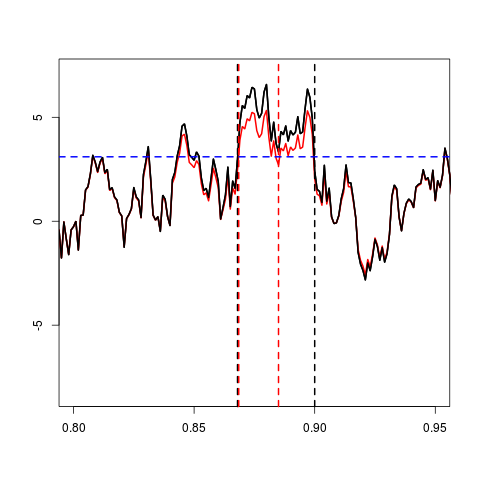
\includegraphics[scale=.4]{../FIGURES/Fig-MinReg-Diffus-Continuity}      
% %     \end{tabular}
% %   \end{tabular}
% 
% }
% 
%====================================================================
\frame{\frametitle{(Provisional) conclusion}

  \paragraph{Pros:}
  \begin{itemize}
  \item An exact importance sampling scheme can be designed \\
  \item The approximation can handle arbitrary loci density $n$ and number of patients $p$ \\
  \ra 'scalable' approach for next sequencing technologies ($n \approx 10^8$)
  \item Abacus can be computed once for all.
  \end{itemize}

  \pause \bigskip \bigskip
  \paragraph{But:}
  \begin{itemize}
  \item The proposed sampling strategy still needs to be implemented in practice...
  \item The efficiency of the preferential sampling scheme is critical.
%   \item   We have no theoretical guarantee that the longest excursion of the process of interest behaves like this of an Ornstein-Uhlenbeck process.
%   \item In the worst case, the proposed approach is useless.
  \end{itemize}

  }

% %====================================================================
% \frame{\frametitle{General conclusion}
% 
%   \paragraph{Running after technologies.}
%   \begin{itemize}
%   \pause
%   \item Each new technology provides new (statistical) problems. \\ ~
%   \pause
%   \item Many of them are related to artifact correction \\
%   \ra Statistical developments become rapidly obsolete.  \\ ~
%   \pause
%   \item Some are more rewarding: \\
%   \ra they raise interesting theoretical problems \\
%   \ra to provide answers to practical questions. 
%   \end{itemize}
% 
% }
% 
%====================================================================
\frame[allowframebreaks]{ \frametitle{References}
{\tiny
  \bibliography{/home/robin/Biblio/ARC,/home/robin/Biblio/AST,/home/robin/Biblio/SSB}
  \bibliographystyle{/home/robin/LATEX/Biblio/astats}
  %\bibliographystyle{plain}
  }
}

%====================================================================
\frame{\frametitle{Constructing the waiting time}
  
  \paragraph{Automaton view-point.} $\ell = 4$:
  $$
  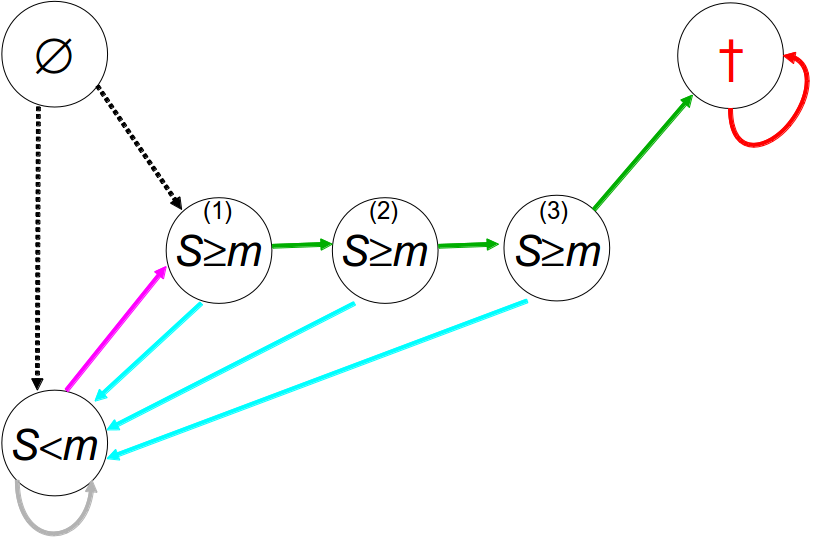
\includegraphics[height=.5\textheight, clip=]{../FIGURES/Fig-MinReg-Automaton}
  $$
  \begin{enumerate}
   \item Construct the transition matrix $\Pt_S$ of this automaton.
   \item Compute $\left[\left(\Pt_S\right)^{n-1}\right]_{S(0), \dagger}$.
  \end{enumerate}
}

%====================================================================
%====================================================================
\end{document}
%====================================================================
%====================================================================

